%\title{LaTeX Portrait Poster Template}
%%%%%%%%%%%%%%%%%%%%%%%%%%%%%%%%%%%%%%%%%
% a0poster Portrait Poster
% LaTeX Template
% Version 1.0 (22/06/13)
%
% The a0poster class was created by:
% Gerlinde Kettl and Matthias Weiser (tex@kettl.de)
% 
% This template has been downloaded from:
% http://www.LaTeXTemplates.com
%
% License:
% CC BY-NC-SA 3.0 (http://creativecommons.org/licenses/by-nc-sa/3.0/)
%
%%%%%%%%%%%%%%%%%%%%%%%%%%%%%%%%%%%%%%%%%

%----------------------------------------------------------------------------------------
%	PACKAGES AND OTHER DOCUMENT CONFIGURATIONS
%----------------------------------------------------------------------------------------

\documentclass[a0,landscape]{a0poster}

\usepackage{multicol} % This is so we can have multiple columns of text side-by-side
\columnsep=100pt % This is the amount of white space between the columns in the poster
\columnseprule=3pt % This is the thickness of the black line between the columns in the poster

\usepackage[svgnames]{xcolor} % Specify colors by their 'svgnames', for a full list of all colors available see here: http://www.latextemplates.com/svgnames-colors

\usepackage{times} % Use the times font
%\usepackage{palatino} % Uncomment to use the Palatino font

% Justify
\usepackage{ragged2e}

% Titles
\usepackage{titlesec}
\titleformat*{\section}{\LARGE\bfseries\filcenter}
\titleformat*{\subsection}{\Large\bfseries\filcenter}
\titleformat*{\subsubsection}{\large\bfseries\filcenter}
\titleformat*{\paragraph}{\large\bfseries\filcenter}
\titleformat*{\subparagraph}{\large\bfseries\filcenter}
\titlespacing\section{0pt}{10pt}{6pt}
\titlespacing\subsection{0pt}{0pt}{0pt}

\usepackage{enumitem}
\newenvironment{nitemize}{%
  \begin{itemize}[topsep=6pt,itemsep=2pt,parsep=0pt]%
}{%
  \end{itemize}%
}
\newenvironment{nenumerate}{%
  \begin{enumerate}[topsep=6pt,itemsep=2pt,parsep=0pt,label=\textbf{\arabic*. }]%
}{%
  \end{enumerate}%
}

\usepackage{graphicx} % Required for including images
\graphicspath{{figures/}} % Location of the graphics files
\usepackage{booktabs} % Top and bottom rules for table
\usepackage[font=small,labelfont=bf]{caption} % Required for specifying captions to tables and figures
\usepackage{amsfonts, amsmath, amsthm, amssymb} % For math fonts, symbols and environments
\usepackage{wrapfig} % Allows wrapping text around tables and figures
\newenvironment{Figure}
  {\par\medskip\noindent\minipage{\linewidth}}
  {\endminipage\par\medskip}

\let\OLDthebibliography\thebibliography
\renewcommand\thebibliography[1]{
  \OLDthebibliography{#1}
  \setlength{\parskip}{0pt}
  \setlength{\itemsep}{0pt plus 0.1ex}
}

\begin{document}

%----------------------------------------------------------------------------------------
%	POSTER HEADER 
%----------------------------------------------------------------------------------------

\begin{figure}[!htb]
\minipage{0.15\textwidth}
  \begin{flushleft}
  
\includegraphics[width=\textwidth,keepaspectratio]{ICL.eps}
  \end{flushleft}
\endminipage\hfill
\minipage{0.7\textwidth}
\centering
\veryHuge \color{Black} \textbf{Decoding of selective attention to continuous speech from the human auditory brainstem response} \color{Black}\\[1cm] % Title
\LARGE \textbf{\underline{Mikolaj A. Kegler}, Octave Etard, Antonio E. Forte, Tobias Reichenbach}\\[0.4cm] % Author(s)
\Large  Department of Bioengineering \& Centre for Neurotechnology, Imperial College London, SW7 2AZ, London, United Kingdom% University/organization
\endminipage\hfill
\minipage{0.15\textwidth}%
  \begin{flushright}
  
\includegraphics[width=\textwidth,keepaspectratio]{CDT.png}
  \end{flushright}
\endminipage
\end{figure}
% \vspace{0.2cm}
% \end{minipage}
%
% \begin{minipage}[b]{0.25\linewidth}
% \includegraphics[width=20cm]{logo.png}\\
% \end{minipage}

%\vspace{0.4cm} % A bit of extra whitespace between the header and poster content

%----------------------------------------------------------------------------------------

\begin{multicols*}{3} % This is how many columns your poster will be broken into, a portrait poster is generally split into 2 columns

%----------------------------------------------------------------------------------------
%	INTRODUCTION
%----------------------------------------------------------------------------------------
\section*{\underline{Introduction}}
\begin{flushleft}
\normalsize
The neural activity of the auditory brainstem tracks features such as the onset of sound or the frequency of a pure tone \cite{Skoe2010}. 
%Continuous, non-repetitive monotone speech may be employed to measure the auditory brainstem response at the fundamental frequency of a speech signal \cite{Reichenbach2016}. Cross-correlation of the fundamental waveform, extracted from natural speech, with the neural response of the auditory brainstem yields a measure of the brainstem's response to natural non-repetitive speech \cite{Forte2017b}.
Continuous, non-repetitive speech may also be employed to measure the auditory brainstem response at the fundamental frequency of a speech signal \cite{Reichenbach2016,Forte2017b}.
These studies employed a few electrodes only, located at the mastoids and at Cz. Here we sought to investigate if the auditory brainstem response to natural speech can also be detected from high-density EEG recordings; this would allow to measure responses from the brainstem as well as from the cortex simultaneously.
\end{flushleft}

%----------------------------------------------------------------------------------------
%	OBJECTIVES
%----------------------------------------------------------------------------------------

\section*{\underline{Objectives}}
\vspace{12pt}
\begin{flushleft}
\normalsize
\begin{nitemize}
\item Establish the methodology for detecting the auditory brainstem response (ABR) to natural speech from high-density EEG recordings.
\item Verify that the ABR to natural speech measured from high-density EEG is modulated by auditory attention \cite{Forte2017b}.
\item Establish the methodology for the on-line decoding of auditory attention based on the ABR detected from high-density EEG recordings.
\end{nitemize}
\end{flushleft}

%----------------------------------------------------------------------------------------
%	MATERIALS AND METHODS
%----------------------------------------------------------------------------------------

\section*{\underline{Materials \& methods}}
%\subsection*{Experimental design}
\vspace{12pt}
\begin{flushleft}
\normalsize
\begin{nitemize}
\item 18 young \& healthy participants.
\item 64-channel EEG sampled at 1 kHz was recorded and band-pass filtered between 100-300 Hz.
\item \textbf{Natural speech stimuli} - audiobook fragments read by male and female speakers.
\item \textbf{Single speaker experiment} - attend to the audiobook fragment read by the female speaker.
\item \textbf{Competing speakers experiment} x2 - attend to one speaker and ignore the other + the opposite.
%\item \textbf{Competing speakers experiment 2} - attend to the second voice and ignore the other.
\end{nitemize}
\end{flushleft}
%\subsection*{Fundamental waveform of speech}
\subsection*{Complex linear modelling}
\begin{Figure}
\minipage{0.5\textwidth}
  \begin{flushleft}
\textbf{The fundamental waveform} (red) is a waveform that vibrates at the time-varying fundamental frequency of natural speech (black). Here, it has been obtained using the method developed in \cite{Forte2017b} and downsampled to 1 kHz to match the sampling frequency of the neural data.
  \end{flushleft}
\endminipage\hfill
\minipage{0.5\textwidth}%
  \centering
  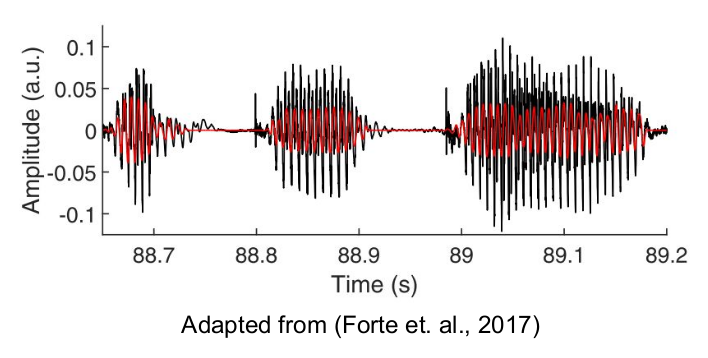
\includegraphics[width=\textwidth,keepaspectratio]{fundamental.png}
\endminipage

%\subsection*{Complex linear models}

% \begin{Figure}
% \minipage{0.75\textwidth}
%   \centering
%   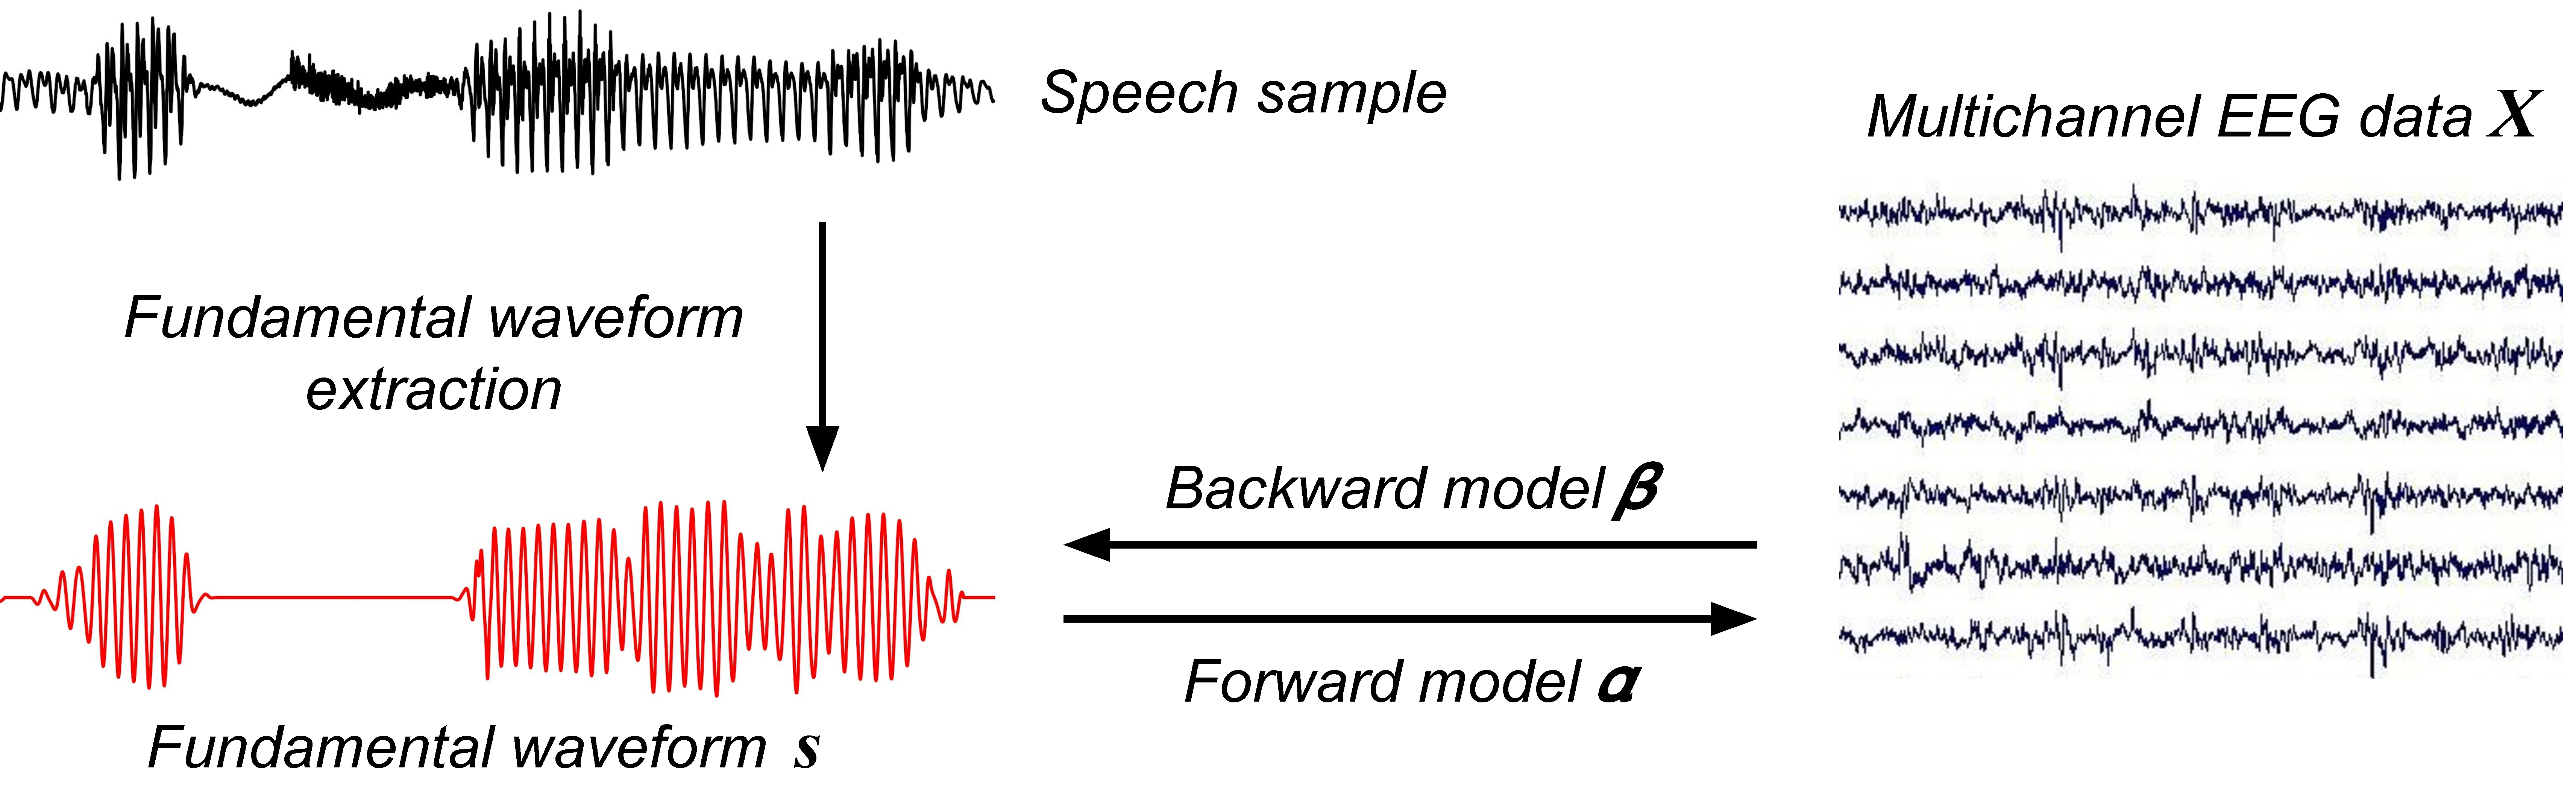
\includegraphics[width=\textwidth,keepaspectratio]{ComplexModel.pdf}
% \endminipage\hfill
% \minipage{0.25\textwidth}%
% \centering
% $f_{a}(t) = f(t) + jH(f(t))$
% $s = X_{a}\beta + \eta$
% $X = s_{a}\alpha + \eta$
% $\beta=(X_{a}^{T}X_{a}+I\lambda)^{-1}X_{a}^{T}s$
% \endminipage
% \end{Figure}
\centering
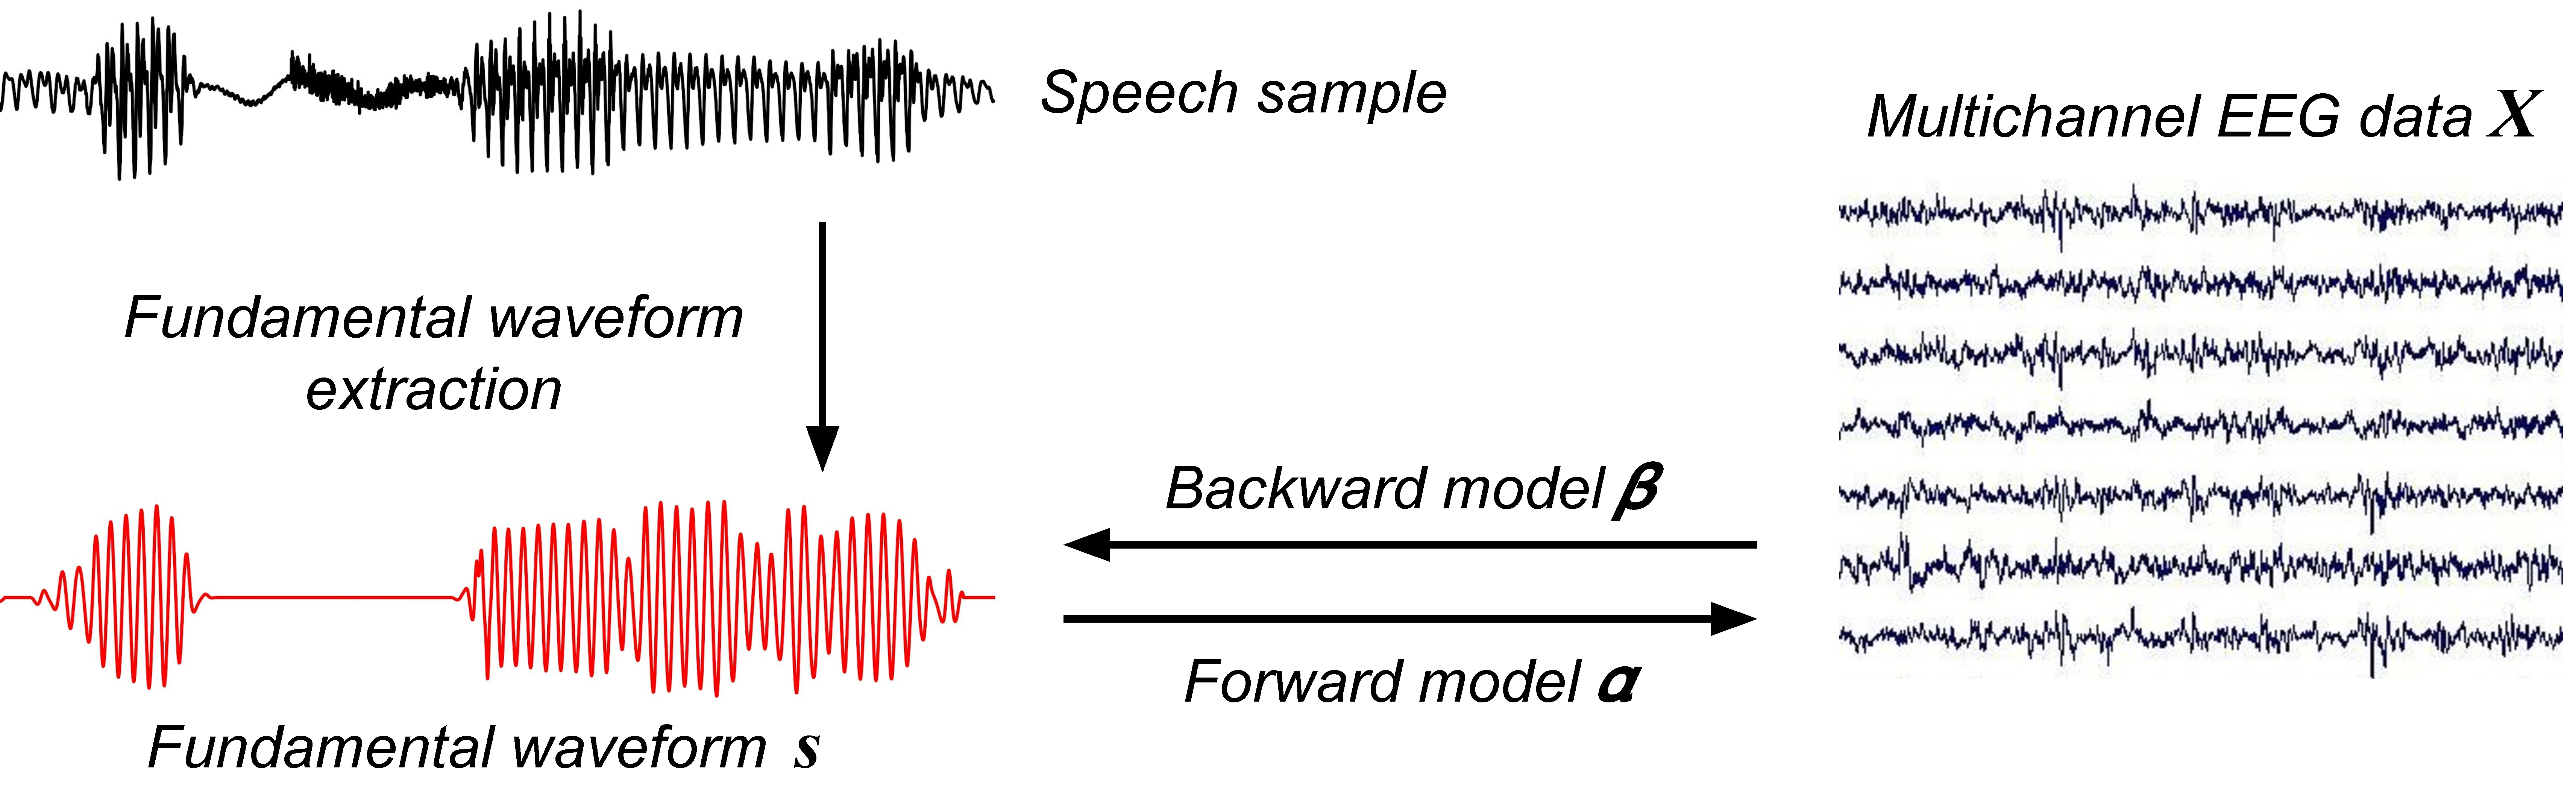
\includegraphics[width=\textwidth,keepaspectratio]{ComplexModel.pdf}
\end{Figure}
\begin{nitemize}
\item \textbf{Analytic signal} - a complex signal, which real and imaginary parts are the original signal ($f(t)$) and its Hilbert transform: $f_{a}(t) = f(t) + jH(f(t))$, where $H$ denotes the hilbert transform.
\item \textbf{Backward model} ($\boldsymbol{\beta}$) maps the analytic signal of the EEG ({$\boldsymbol{X}_{a}$}) to the fundamental waveform ($\boldsymbol{s}$).
\item \textbf{Forward model} ($\boldsymbol{\alpha}$) maps the analytic signal of the fundamental waveform ({$\boldsymbol{s}_{a}$}) to the EEG ($\boldsymbol{X}$).
\item \textbf{Complex coefficients} of the models were acquired via regularized linear regression.
%\item \textbf{The reconstruction accuracy} of the backward models is measured through \textbf{Pearson’s correlation coefficient} between the predicted and the actual data in \textbf{five-fold cross-validation}.
\end{nitemize}

\subsection*{Auditory attention decoding}
\vspace{14pt}
\begin{nitemize}
%\item \textbf{Goal}: determine which voice is attended by the participant in the competing speakers experiments based on the neural activity recorded with EEG.
\item \textbf{The speaker-specific decoding} employed the four unique backward models that estimated the fundamental waveforms of the male voice while it was attended (\textbf{MA}) or ignored (\textbf{MI}) and the female voice while it was attended (\textbf{FA}) or ignored (\textbf{FI}).
\item \textbf{The speaker-independent decoding} employed the two backward models that were trained to reconstruct any given attended (\textbf{A}) or ignored (\textbf{I}) voice, regardless of the identity of the speaker.
%\item \textbf{The 'out-of-the box' models} are trained on the pooled data from \textbf{all participants but one}, that serve as a testing set when evaluating the model in a cross-validation fashion.
\item \textbf{The auditory attention} was determined from the reconstruction accuracies of the models by setting an arbitrary classification boundary in the feature space.
\end{nitemize}

%----------------------------------------------------------------------------------------
%	RESULTS
%----------------------------------------------------------------------------------------

\section*{\underline{Results}}

\subsection*{Detection of the ABR in the single speaker experiment}
\begin{Figure}
\centering
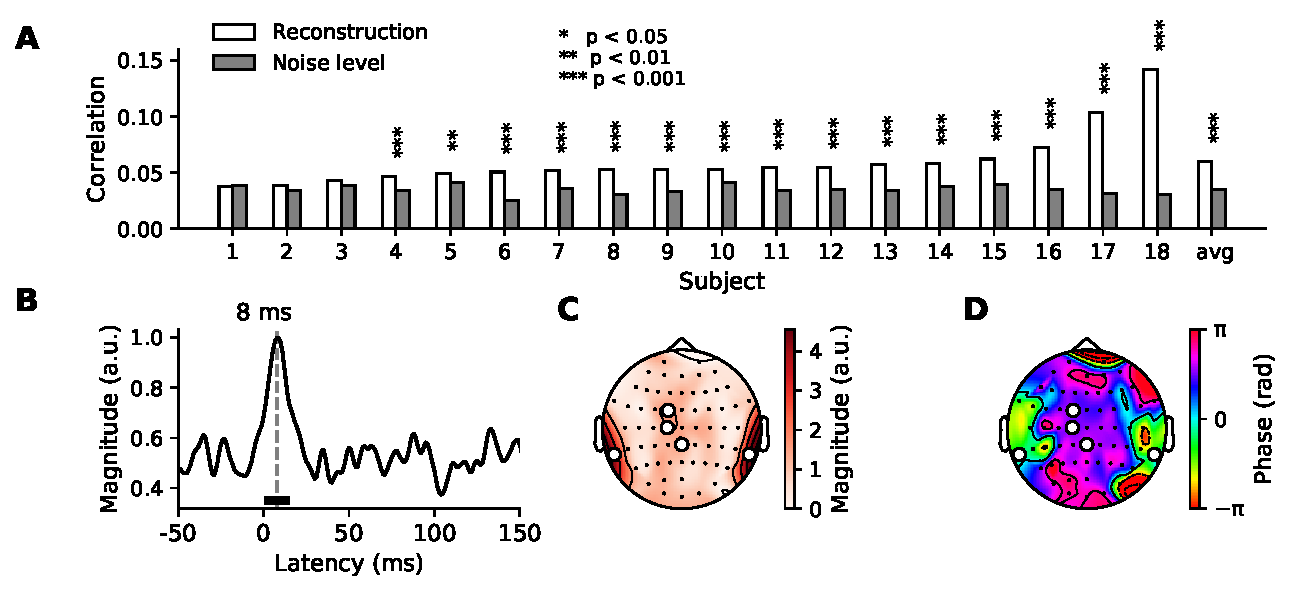
\includegraphics[width=\linewidth,keepaspectratio]{Figure_1.pdf}
\end{Figure}
\begin{flushleft}
The channel-averaged magnitude of the complex forward model reflects the latency of the dominant brain response. The latency of \textbf{8 ms} indicated the brainstem activity (\textbf{A}). At the latency of 8 ms, electrodes located at \textbf{mastoids} and at \textbf{the centre of a scalp} (white disks) yielded significantly higher magnitudes, as compared to the models estimating the noise level (\textbf{C}).
\end{flushleft}

% \begin{Figure}
% \centering
% 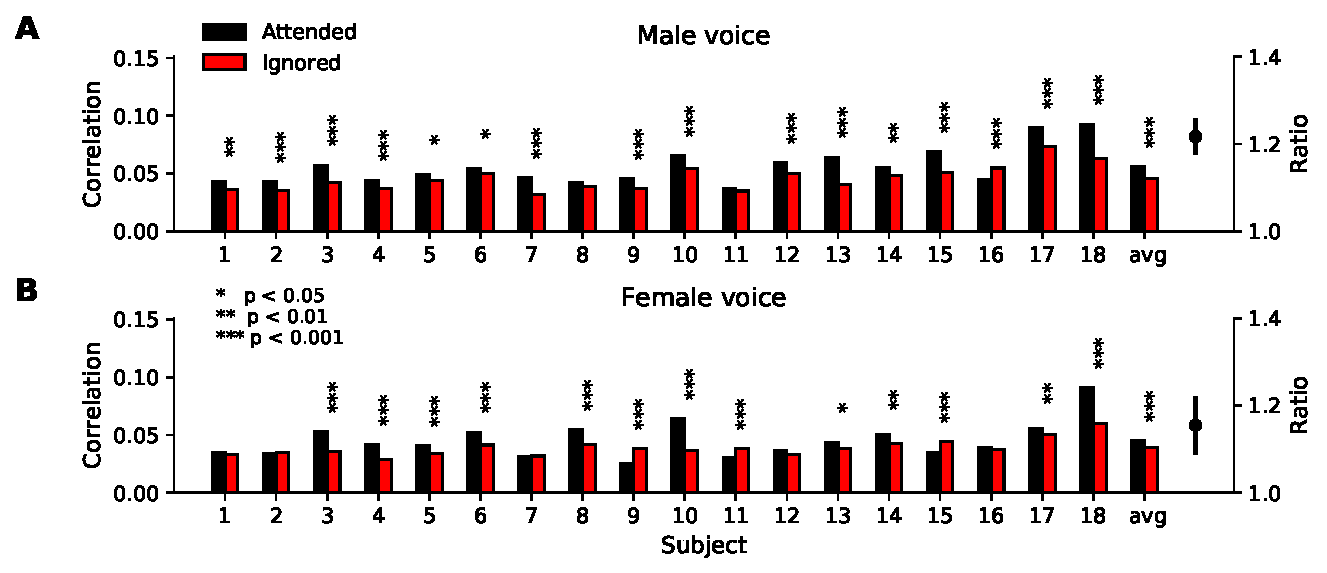
\includegraphics[width=0.5\linewidth,keepaspectratio]{Figure_2.pdf}
% \end{Figure}

\subsection*{Attentional modulation of the detected ABR}
\begin{Figure}
\centering
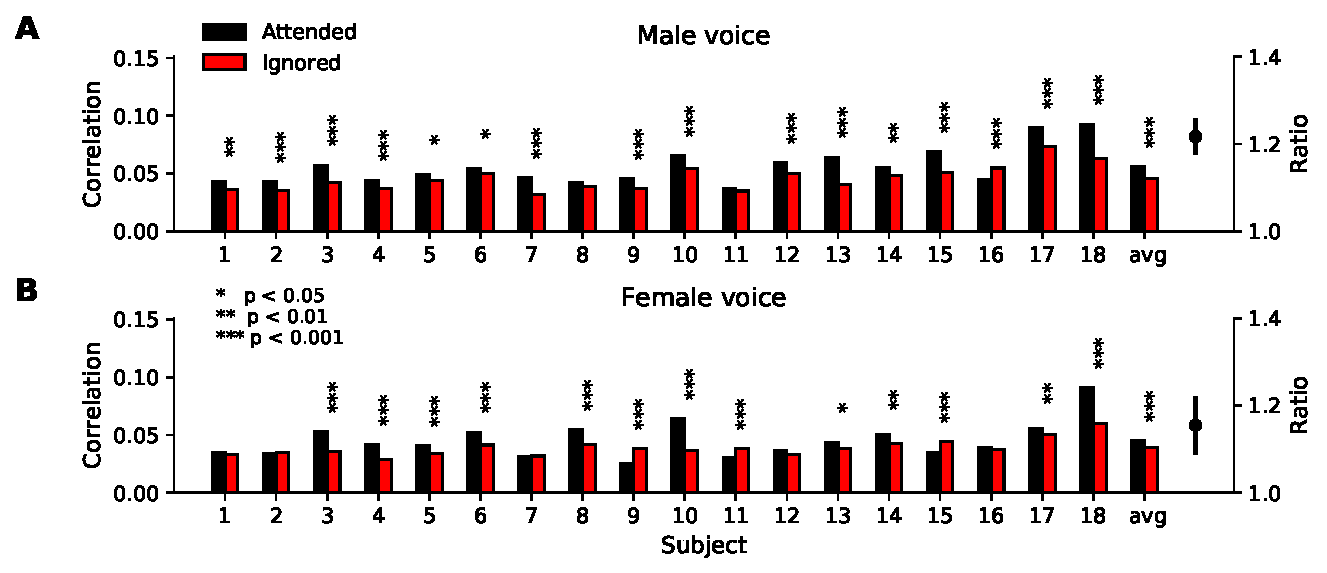
\includegraphics[width=\linewidth,keepaspectratio]{Figure_3.pdf}
\end{Figure}
\begin{flushleft}
Complex backward models trained to reconstruct given voice when it was \textbf{attended} (black) yielded significantly higher correlations for the majority of subjects. The averaged reconstruction ratios of the attended and ignored models were significantly greater than unity indicating consistent \textbf{attentional modulation} of the detected ABR across the participants.
\end{flushleft}

\subsection*{Comparison of the attended and ignored speaker-specific models}
\minipage{0.65\linewidth}
\begin{Figure}
\begin{flushright}
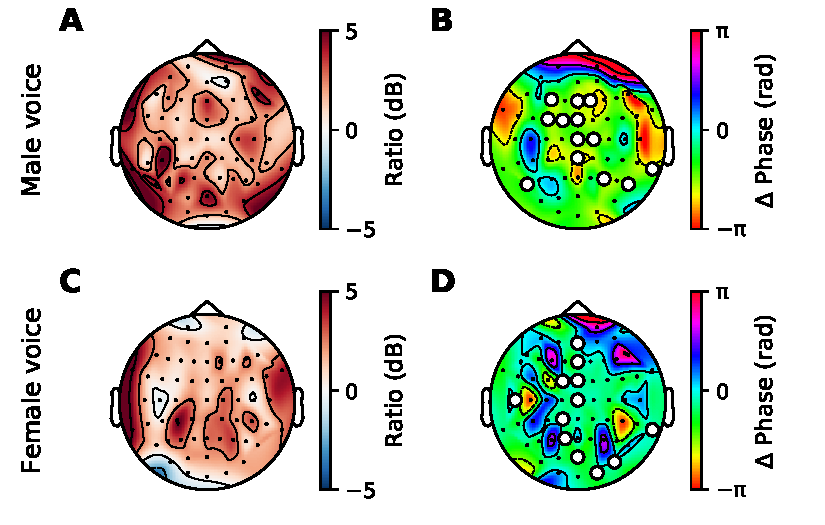
\includegraphics[width=\linewidth,keepaspectratio]
{Figure_4.pdf}
\end{flushright}
\end{Figure}
\endminipage\hfill
\minipage{0.35\linewidth}
\begin{flushleft}
To characterize the neural mechanism underlying the attentional modulation of the detected brainstem responses, the forward models for the attended and ignored voices were compared. The magnitudes of the models \textbf{did not differ significantly} across the participants (\textbf{A}, \textbf{C} averaged ratios). However, the channels located at mastoids and at the centre of a scalp yielded consistent, significant \textbf{phase difference} across the participants (\textbf{B}, \textbf{D}, white disks).
\end{flushleft}
\endminipage\hfill

\subsection*{Speaker-specific auditory attention decoding}
\vspace{0.7cm}
\minipage{0.7\linewidth}
\begin{Figure}
\centering
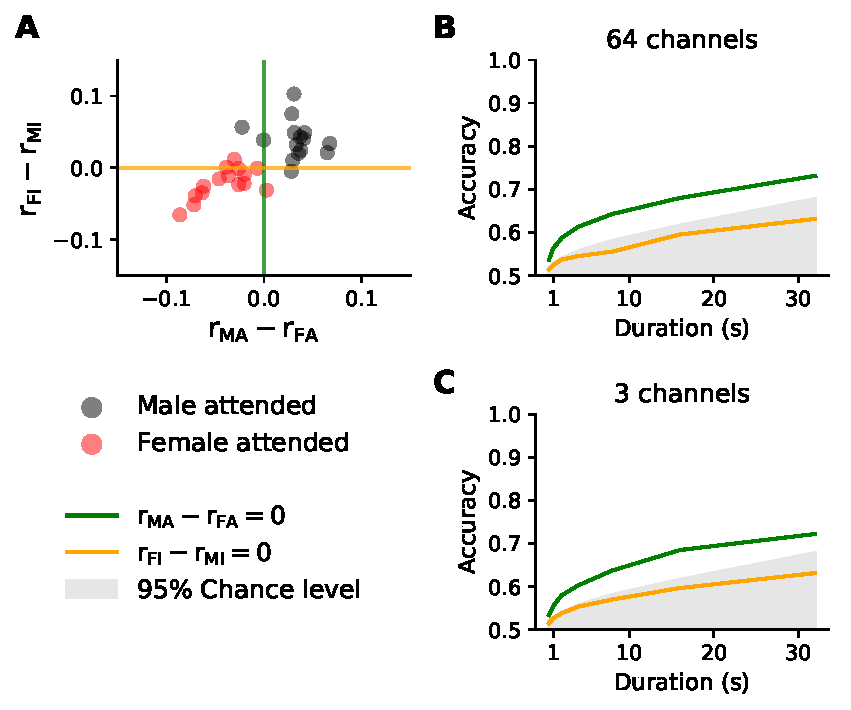
\includegraphics[width=\linewidth,keepaspectratio]{Figure_5.pdf}
\end{Figure}
\endminipage\hfill
\minipage{0.3\linewidth}
\begin{flushleft}
Auditory brainstem responses detected from high-density EEG allowed for the classification of auditory attention in the competing speakers task employing continuous speech. For each segment of testing data, reconstructions accuracies (\textbf{r}) of the two attended (\textbf{MA}, \textbf{FA}) and the ignored (\textbf{FI}, \textbf{MI}) models were subtracted. Arbitrary boundaries in the feature space reflected classification based on the attended (green) or the ignored models (orange). Classification based on \textbf{only 3 EEG channels} (TP9, TP10, Cz) (\textbf{C}) yielded comparable results to that achieved using all 64 (\textbf{B}).
\end{flushleft}
\endminipage\hfill
\vspace{0.5cm}

\subsection*{Alternative setups for the auditory attention decoding}
\begin{Figure}
\centering
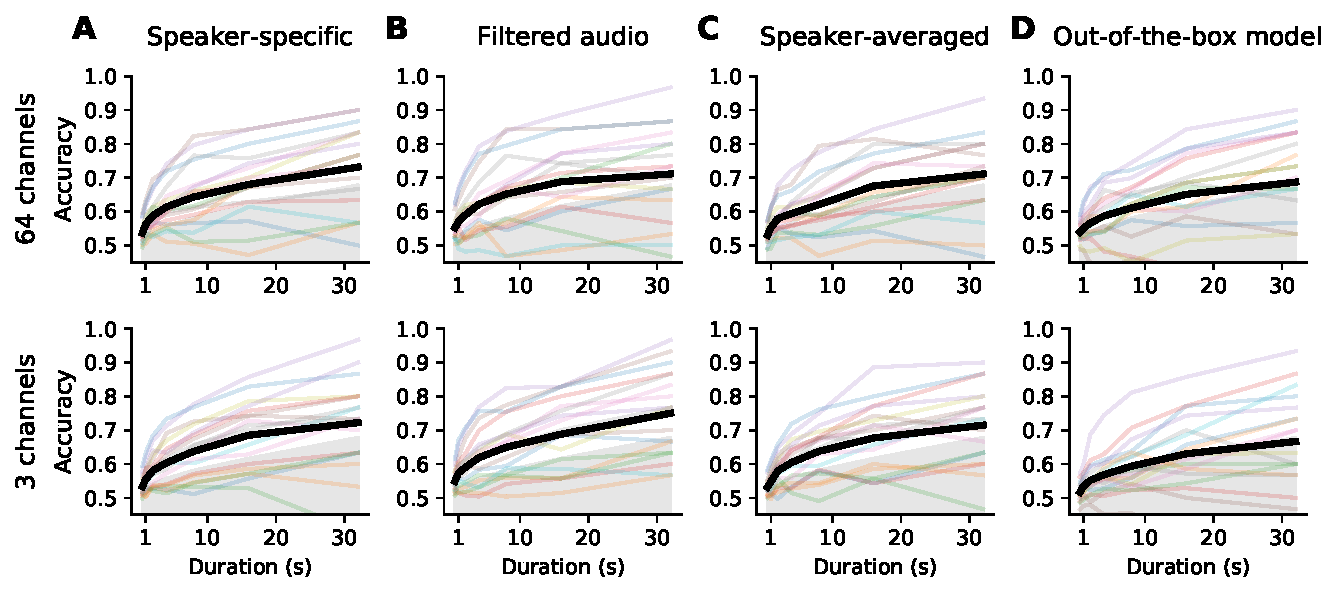
\includegraphics[width=\linewidth,keepaspectratio]{Figure_6.pdf}
\end{Figure}
\begin{flushleft}
Coloured traces represent single-subject results and the thicker black lines illustrate the population averages. The substitution of the fundamental waveform, employed in the proposed complex modelling approach, for the \textbf{bandpass filtered} (between 100 and 300 Hz) \textbf{speech signal} did not decrease the speaker-specific decoding accuracy (\textbf{B}). The simple algorithm employing the \textbf{speaker-independent backward models}, trained on the concatenated data across the two competing speakers tasks, did not influence the averaged attention decoding accuracy either (\textbf{C}). The classifier based on the \textbf{\textit{Out-of-the-box}}, population-averaged backward models (\textbf{D}) performed significantly above the chance level. It suggests consistency of the attentional modulation of the detected brainstem responses among the participants.
\end{flushleft}

%----------------------------------------------------------------------------------------
%	ACKNOWLEDGEMENTS
%----------------------------------------------------------------------------------------

\small
\subsection*{Acknowledgements}
\begin{flushleft}
The original script for extracting the fundamental waveform from speech samples has been acquired from A. E. Forte \cite{Forte2017b}. The EEG data have been obtained by O. Etard.
\end{flushleft}

%----------------------------------------------------------------------------------------
%	REFERENCES
%----------------------------------------------------------------------------------------
\subsection*{References}
\begingroup
\footnotesize
\renewcommand{\section}[2]{}%
\bibliographystyle{apalike}
\bibliography{Mendeley}
\endgroup
%----------------------------------------------------------------------------------------

\end{multicols*}
\end{document}